\section{Selecting by a threshold}
\label{app:thresholds}
The examples are those of Figure~\ref{fig:other-recall}. Precision, recall and F1 pool the options of all examples.

\begin{figure*}[h]
\centering
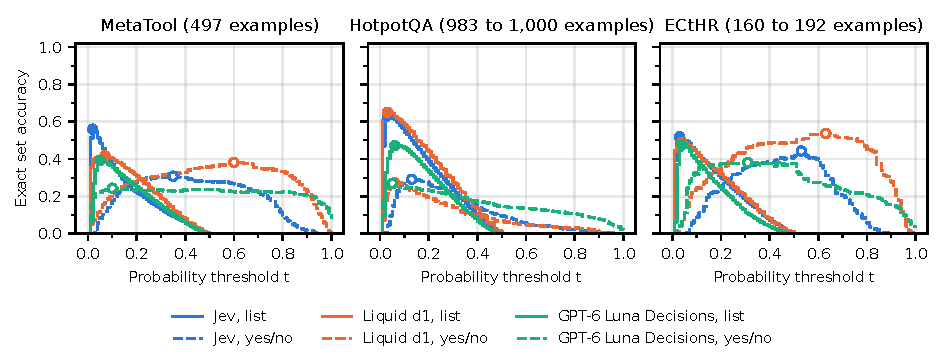
\includegraphics[width=\linewidth]{figures/exact_set}
\caption{Exact set accuracy: the share of examples in which every correct option is at or above the threshold $t$ and every distractor is below it. Above 0.50 the list curves are 0 by construction.}
\label{fig:exact-set}
\end{figure*}

\begin{figure*}[h]
\centering
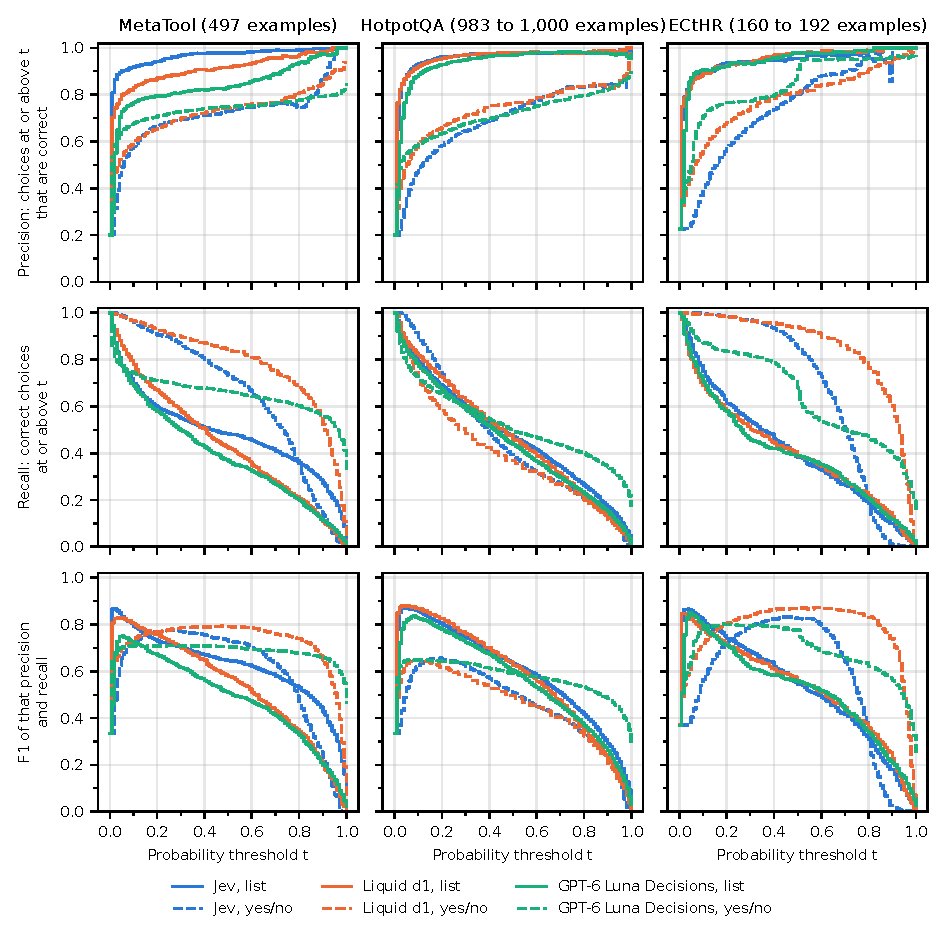
\includegraphics[width=\linewidth]{figures/threshold_measures}
\caption{Precision (the share of options at or above $t$ that are correct), recall (the share of correct options at or above $t$) and their F1. At 0.25 the list has a precision of 0.80 to 0.96 and a recall of 0.51 to 0.67. One correct option per example gives a recall of 0.50 on MetaTool and HotpotQA and about 0.44 on ECtHR.}
\label{fig:threshold-measures}
\end{figure*}
